\chapter{Theoretical Background}\label{chap:theory}

\section{Plasma Generation and Composition}

\subsection{Cathode Spot Plasma Generation}

Cathodic arc plasmas form at microscopic emission centers, known as cathode spots, on an otherwise cold metal electrode under vacuum. Spot ignition occurs when the local cathode surface, through breakdown of adsorbates or field-enhanced thermionic emission, undergoes a rapid, explosive release of electrons and vaporized metal. During a single spot pulse, a few nanograms of the cathode material rapidly heat up, vaporize, and ionize, producing a dense, quasineutral plasma plume composed mostly of metal ions and electrons. The peak spot current densities reach \(10^{10}\)--\(10^{12}\)\,A\,m\(^{-2}\), far above steady-state thermionic or field emission limits. These microexplosions, termed ectons (explosive electron emission centers), were first described by Mesyats \cite{mesyats1995} and produce localized nanosecond-scale plasma bursts. The arc is sustained by repetitive ecton events occurring at or near the same location \cite[Chap.~3.3--3.4]{cathodic_arcs}.




Key Characteristics of Spot-Generated Plasma:
\begin{compactitem}
    \item High degree of ionization: >90 \% of the ejected metal atoms emerge as ions, a consequence of the extreme power density in the cathode spot \cite[Chap.~3.5]{cathodic_arcs}.
    \item Multiply charged ions: the charge state distributions extend to \(Q=3\)–4 for refractory metals, such as Ti and Al, due to the high electron temperature and density in the spot plasma \cite[Chap.~3.5]{cathodic_arcs}.
\end{compactitem}

Spot ignition and quenching occur on timescales of 10--100\,ns, with each pulse ejecting a fully ionized burst of metal vapour. The sustained arc discharge thus consists of continuously overlapping microplasma pulses, producing a metal-rich, high-flux ion stream well-suited for energetic thin-film deposition.


\begin{figure}[h]
	\centering
	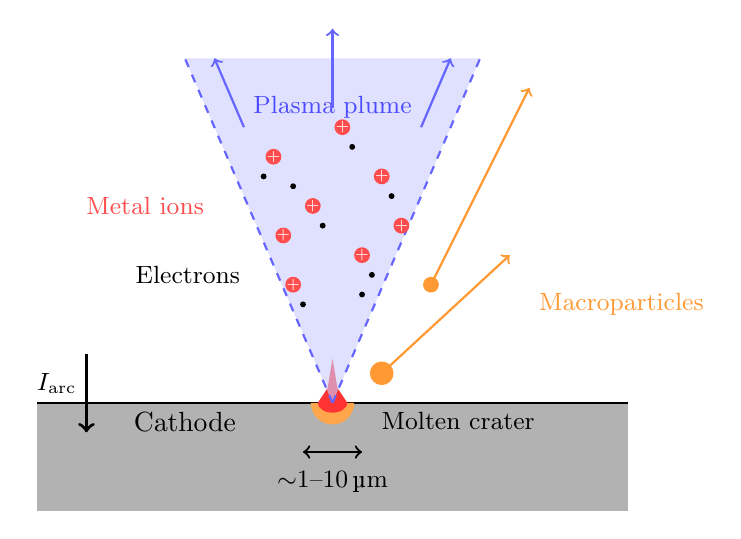
\begin{tikzpicture}[scale=1.25]
		% Cathode block
		\fill[gray!60] (-3,-1.1) rectangle (3,0);
		\draw[thick] (-3,0) -- (3,0);
		\node[below] at (-1.5,0) {Cathode};
		
		% Molten crater
		\fill[orange!70] (-0.22,0) arc (180:360:0.22) -- cycle;
		\fill[red!80] (-0.15,0) arc (180:360:0.15 and 0.1) -- (0.15,0) -- (0.05,0.15) -- (0,0.45) -- (-0.05,0.15) -- (-0.15,0) -- cycle;
		\node[below right, font=\small] at (0.4,0) {Molten crater};
		
		% Plasma plume (expanding cone)
		\fill[blue!20, opacity=0.6] (0,0) -- (-1.5,3.5) -- (1.5,3.5) -- cycle;
		\draw[blue!60, thick, dashed] (0,0) -- (-1.5,3.5);
		\draw[blue!60, thick, dashed] (0,0) -- (1.5,3.5);
		\node[blue!70, font=\small] at (0,3) {Plasma plume};
		
		% Ions (circles with + signs)
		\foreach \x/\y in {-0.4/1.2, 0.3/1.5, -0.2/2.0, 0.5/2.3, -0.6/2.5, 0.1/2.8, 0.7/1.8, -0.5/1.7} {
			\fill[red!70] (\x,\y) circle (0.08);
			\node[white, font=\tiny] at (\x,\y) {+};
		}
		\node[red!70, right, font=\small] at (-2.6,2.0) {Metal ions};
		
		% Electrons (small dots)
		\foreach \x/\y in {-0.3/1.0, 0.4/1.3, -0.1/1.8, 0.6/2.1, -0.7/2.3, 0.2/2.6, -0.4/2.2, 0.3/1.1} {
			\fill[black] (\x,\y) circle (0.03);
		}
		\node[right, font=\small] at (-2.1,1.3) {Electrons};
		
		% Macroparticle (larger droplet trajectory)
		\fill[orange!80] (0.5,0.3) circle (0.12);
		\draw[->, thick, orange!80] (0.5,0.3) -- (1.8,1.5);
		\fill[orange!80] (1,1.2) circle (0.08);
		\draw[->, thick, orange!80] (1,1.2) -- (2,3.2);
		\node[orange!80, right, font=\small] at (2.0,1.0) {Macroparticles};
		
		% Current flow arrow
		\draw[->, very thick] (-2.5,0.5) -- (-2.5,-0.3);
		\node[left, font=\small] at (-2.5,0.2) {$I_{\rm arc}$};
		
		% Spot diameter indicator
		\draw[<->, thick] (-0.3,-0.5) -- (0.3,-0.5);
		\node[below, font=\small] at (0,-0.6) {$\sim$1--10\,\textmu m};
		
		% Expansion arrows
		\draw[->, thick, blue!60] (0,3.0) -- (0,3.8);
		\draw[->, thick, blue!60] (-0.9,2.8) -- (-1.2,3.5);
		\draw[->, thick, blue!60] (0.9,2.8) -- (1.2,3.5);
		
	\end{tikzpicture}
	\caption[Schematic of cathode spot operation]{Schematic of cathode spot operation. The arc current $I_{\rm arc}$ concentrates at a microscopic spot (1--10\,\textmu m diameter), creating a molten crater from which a plasma plume of metal ions, electrons and macroparticles expand. Adapted from \cite{juttner2001}}.
	\label{fig:cathode_spot}
\end{figure}

\subsection{Pulsed vs. Continuous Arc Operation}

Cathodic arcs can operate in either continuous (DC) or pulsed mode, with fundamental differences in plasma generation dynamics. In DC operation, the cathode spot moves continuously across the surface, maintaining a steady-state plasma density determined by the balance between plasma generation at the spot and losses through expansion. The time-averaged plasma properties remain constant, and the ion flux to the substrate is continuous.\\

In pulsed operation, the arc is periodically initiated and extinguished, creating discrete plasma bursts separated by periods with no plasma generation. During the active phase of each pulse, the instantaneous plasma density can be significantly higher than in DC arcs operating at the same average power, because the energy is concentrated in short time intervals. The peak plasma density scales with the instantaneous arc current, which can reach several hundred amperes during the pulse. Between pulses, the plasma expands and dissipates, allowing the cathode surface to cool. This temporal modulation affects both the spot dynamics and the resulting plasma composition.\\

The ion charge state distributions in pulsed arcs are typically similar to or slightly enhanced compared to DC arcs, as the higher instantaneous power density can promote additional ionization events in the cathode spot region \cite[Chap.~10]{cathodic_arcs}. Understanding these temporal plasma dynamics is essential when interpreting flux measurements and correlating them with film growth processes.

\subsection{Plasma Expansion and Macroparticle Filtering}

Following their generation at the cathode spots, the plasma bursts expand into the vacuum chamber. This expansion is supersonic, with ions carrying directed kinetic energy away from the cathode. In many industrial and research systems, the expanding plasma is guided through a magnetic macroparticle filter that removes macroparticles while allowing plasma to pass along curved magnetic field lines.

In the region near the cathode (within a few centimetres of the spot), plasma densities are on the order of \(10^{18}\)\,cm\(^{-3}\) and electron temperatures \(T_e \approx 5\)--10\,eV. As the plume propagates, its density decreases according to
\begin{equation}
	n(r) = \frac{C\,I_{\rm arc}}{r^2}
\end{equation}
where \(I_{\rm arc}\) is the arc current, $r$ the distance, and $C$ a constant related to the ion erosion rate of the cathode material. This \(1/r^2\) scaling assumes free expansion, but deviations can occur due to magnetic fields, collisions, or reactive gases, which may alter the plasma trajectory or cause recombination \cite[Chap.~4.3; Eq.~4.3, p.~178]{cathodic_arcs}.

In cathodic arc discharges from titanium cathodes, whether pure Ti or Ti--Al compounds, ions generally carry an average charge state \(\langle Q\rangle \approx 2.1\)--2.2 at the source \cite[Chap.~4.1; App.~B.8]{cathodic_arcs}. This high degree of ionization reflects the extreme power density of the spot and follows the cohesive energy rule, which links \(\langle Q\rangle\) to the cohesive energy of the cathode material \cite[App.~B.8]{cathodic_arcs}.

In the present work, a 90$^\circ$ curved magnetic filter guides the expanding plasma toward the substrate region while removing macroparticles. After passing through the filter, the plasma has evolved from its initial state at the cathode spot, having undergone expansion, potential collisions with background gas, and interaction with guiding magnetic fields. The properties of this filtered plasma in the substrate region determine the energy and flux delivered to the growing film, and are the focus of the following sections.


%Applying an external axial magnetic field at the source (the “EM-coil” configuration) can boost ⟨Q⟩ by 10–30 \% and increase total ion flux by up to an order of magnitude. Effects attributed to enhanced magnetic insulation and longer plasma spot interaction times \cite{decoupling_kalanov_2025}. In contrast, imposing a DC bias on the source raises the ions’ kinetic energy with minimal change to ⟨Q⟩ or flux, offering a route to decouple kinetic and potential-energy contributions in film-growth studies.\\

\section{Ion Energies and Flux in the Substrate Region}

This section focuses on the properties of ions in the plasma after expansion and filtering, in the region where they reach the substrate and form the growing film.


\subsection{Ion Energies: Origins and Implications}\label{section:ion_energies}

Ions in cathodic arc plasmas carry both kinetic and potential energy. The kinetic energy \(E_{\rm kin}\) arises from the supersonic expansion of plasma from the cathode spot, while the potential energy \(E_{\rm pot}\) is released upon neutralization at the substrate surface and is determined by the ionization states of the ion.

The total energy delivered by an ion to the growing film is
\begin{equation}
	E_{\rm tot} = E_{\rm kin} + E_{\rm pot}.
\end{equation}

For cathodic arc plasmas, the kinetic energy is closely linked to the arc burning voltage, which remains nearly constant at 20--25\,V for most metallic cathodes \cite[Chap.~4.2]{cathodic_arcs}. This voltage accelerates ions away from the cathode region, giving them characteristic drift velocities. As ions traverse the expanding plasma, they may undergo collisions that modify their energy distribution.

Table~\ref{tab:ion_properties} summarizes characteristic ion properties for Ti and Al cathodic arc plasmas in vacuum, measured near the cathode.

\begin{table}[htbp]
	\centering
	\caption[Characteristic ion properties for Ti and Al]{Characteristic ion properties for Ti and Al cathodic arc plasmas in vacuum, near the cathode \cite[App.~B; Table~B.8]{cathodic_arcs}.}
	\label{tab:ion_properties}
	\begin{tabular}{lcccc}
		\toprule
		Species & $\langle Q \rangle$ & $E_{\rm kin}$ (eV) & $E_{\rm pot}$ (eV) & $E_{\rm tot}$ (eV) \\
		\midrule
		Ti$^{2+}$ & 2.1 & 59 & 21 & 80 \\
		Al$^{2+}$ & 1.7 & 28 & 24 & 52 \\
		\bottomrule
	\end{tabular}
\end{table}


These values, measured near the cathode spot, serve as reference for understanding the energy budget of ions. In this work, the plasma is characterized after expansion and filtering, where ion energies may differ from these initial values due to collisions and field effects. Nonetheless, for the materials used in this work, the total ion energies are expected to exceed the approximately 30\,eV threshold for subplantation, enabling densification and improved crystallinity in Ti--Al--N films without requiring external substrate heating \cite[Chap.~8.1--8.2]{cathodic_arcs}.


\subsection{Effect of Distance on Ion Properties}

As ions travel from the cathode through the filter and toward the substrate, their properties evolve due to geometric expansion and potential collisions. The ion flux decreases with the square of the distance due to the expanding plasma front. Additionally, collisions with background gas (if present) can reduce ion kinetic energies and alter charge state distributions through charge-exchange reactions.\\

In vacuum (metallic mode), the ion energy distributions remain relatively narrow and well-defined. At increased distances, the plasma density decreases but the relative composition and charge states are largely preserved. However, the ion flux at the substrate position becomes a critical parameter, as it determines the rate at which energy is delivered to the growing film. Understanding how distance affects the ion flux therefore provides insight into the spatial uniformity of the deposition process and allows optimization of substrate positioning.

\subsection{Effect of External Magnetic Fields}

Applying an external axial magnetic field at the arc source modifies the plasma properties in several ways. Enhanced magnetic insulation prolongs the interaction time between electrons and ions in the cathode spot region, leading to:
\begin{compactitem}
	\item Increased average ion charge state \(\langle Q \rangle\), which increases the ion potential energy,
	\item Simultaneously increased ion kinetic energy,
	\item Enhanced ion flux, which can increase by up to an order of magnitude \cite{RN5}.
\end{compactitem}

These effects are inherently coupled: the external magnetic field simultaneously increases both the ion charge states (and thus potential energy) and the total ion flux. This coupling presents a challenge for isolating the individual contributions of ion energy and ion flux to film growth. Decoupling these parameters requires additional experimental approaches, such as varying the source-to-substrate distance to modulate flux while maintaining similar ion energies, or applying bias voltages to shift ion kinetic energies independently \cite{unutulmazsoy,decoupling_kalanov_2025}. The interplay between magnetic field strength, ion flux, and ion energy forms a central theme of this work.



\subsection{Ion Flux}
\label{section:ion_flux}

The ion flux $\Gamma$ represents the number of ions arriving per unit area per unit time, expressed in ions\,cm$^{-2}$\,s$^{-1}$. In a multiply charged plasma, the total measured ion current density $J_i$ (A\,cm$^{-2}$) relates to $\Gamma$ via
\begin{equation}
	\Gamma = \frac{J_i}{e\,\langle Q \rangle},
\end{equation}
where $e$ is the elementary charge and $\langle Q \rangle$ the average ion charge state. This relationship is central to correlating time-averaged ion flux with deposited mass.

In vacuum cathodic arcs, the burning voltage remains nearly constant at 20--25\,V for arc currents up to 1\,kA, so the plasma generation rate and thus $\Gamma$ increases approximately linearly with $I_{\rm arc}$ \cite[Chap.~6.5]{cathodic_arcs}. However, the absolute ion flux at the substrate depends not only on the arc current but also on the distance from the source and the presence of magnetic fields or reactive gases. These factors determine the fraction of generated plasma that reaches the substrate and the composition of that plasma. The transition from metallic to reactive operation introduces additional complexity, as discussed in the following section.

\section{Reactive Mode and Nitrogen Activation}

\subsection{Transition from Metallic to Reactive Mode}

Cathodic arc deposition operates in two distinct regimes. In metallic mode, the cathode surface remains uncovered and the plasma consists exclusively of metal ions, characterized by high ionization degrees. In reactive mode, a background gas such as N$_2$ adsorbs onto the cathode surface, forming a compound layer that poisons the cathode and alters both spot behaviour and plasma composition \cite[Chap.~9.2]{cathodic_arcs}.

When N$_2$ is introduced, a dynamic equilibrium develops between compound formation (through adsorption and reaction at the cathode surface) and compound removal (via explosive ecton events that eject both metal and nitride fragments) \cite[Chap.~9.3]{cathodic_arcs}. The equilibrium position depends on gas pressure, arc current, and cathode composition. At low N$_2$ pressures or high power densities, type-2 (metal-rich) spots prevail, maintaining predominantly metal ion flux. At higher pressures, type-1 (poisoned) spots dominate, producing a mixed plasma of metal and nitrogen ions \cite[Chap.~9.4]{cathodic_arcs}. This transition affects not only the chemical composition of the deposited film but also the energy distribution and charge state distribution of the plasma, as compound formation at the cathode alters the electron emission and plasma generation mechanisms.


\subsection{Activated Nitrogen Species}

In reactive mode, the plasma contains not only metal ions but also activated nitrogen species. These include:
\begin{compactitem}
	\item Ionized nitrogen: N$^+$ and N$_2^+$ ions formed by electron-impact ionization,
	\item Neutral but excited nitrogen: metastable N$_2$ and atomic N species that carry internal energy but no net charge.
\end{compactitem}

The term ``activated nitrogen'' encompasses both ionic and neutral excited species that participate in film growth. While ionized species can be detected directly by mass spectrometry, the contribution of neutral activated species is more difficult to quantify. This distinction is important because the total deposited flux includes both ionic and neutral components, whereas ion current measurements detect only the charged fraction.

Charge exchange with N$_2$ reduces the average charge state of metal ions and introduces gas-ion species, altering the potential energy delivered to the film \cite[Chap.~9.4]{cathodic_arcs}. Collisions during plasma expansion also reduce ion drift velocities, lowering kinetic energy before substrate impact. These effects collectively modify the energy budget available for film growth in reactive mode compared to metallic mode. The interplay between metal ion flux, activated nitrogen flux, and their respective energies determines the resulting film composition, structure, and properties, as discussed in the following section.


\section{Plasma--Surface Interactions and Film Growth}

\subsection{Energetic Condensation and Subplantation}

When metal ions with sufficient energy strike the growing film, they penetrate below the surface and deposit energy through a shallow collision cascade. This subplantation process produces two key effects:

\begin{compactitem}
	\item \textbf{Localized densification:} Ions with energies above approximately 30\,eV implant beneath the surface, occupying interstitial sites and displacing near-surface atoms through knock-on collisions. This reduces porosity and increases film density, which is particularly important for transition-metal nitride coatings such as Ti--Al--N \cite[Chap.~8.1]{cathodic_arcs}.
	
	\item \textbf{Atomic-scale heating:} The deposition of kinetic energy and release of potential energy (ionization enthalpy) generate localized, nanosecond-scale temperature spikes. These enhance adatom mobility and promote crystallite coalescence without requiring global substrate heating \cite[Chap.~8.2]{cathodic_arcs}.
\end{compactitem}

As the energetic input from ions increases, films transition from porous, amorphous structures to dense, crystalline coatings. This densification introduces compressive stresses of several GPa through atomic peening \cite[Chap.~8.1--8.4]{cathodic_arcs}. For example, TiN films grown with total ion energies of approximately 60\,eV develop a preferred cubic (111) texture and hardness exceeding 30\,GPa.

The relationship between ion flux and film growth rate is dependent on
\begin{equation}
	R = \frac{m_{\rm ion}\,\Gamma\,S}{\rho_{\rm film}},
\end{equation}
where $m_{\rm ion}$ is the average ion mass, $\Gamma$ the ion flux, $S$ the sticking coefficient, and $\rho_{\rm film}$ the film density. The sticking coefficient $S$ represents the probability that an arriving ion incorporates into the growing film rather than being reflected or resputtered; for metal ions at moderate energies (below the resputter threshold of approximately 100--200\,eV), $S \approx 1$. However, the film density $\rho_{\rm film}$ itself depends on the ion energy and flux, as higher energies promote densification through subplantation. This interdependence between flux, energy, and resulting film structure motivates the systematic study of these parameters, which is the focus of this work.



\subsection{Structure-Zone Models}

The microstructure of thin films deposited by physical vapour deposition depends strongly on the energy and flux of incident species. Thornton's structure-zone model, originally developed for magnetron sputtering, relates film morphology to the homologous temperature $T/T_m$ (substrate temperature normalized to the melting point) and working gas pressure \cite{thornton1977}. At low $T/T_m$ and high pressures, films exhibit porous, columnar structures (Zone~1) due to limited adatom mobility. As $T/T_m$ increases, denser columnar (Zone~T) and eventually equiaxed crystalline structures (Zone~2 and Zone~3) develop.

Anders extended this framework to account for the energetic ion bombardment characteristic of cathodic arc deposition \cite{anders2010szm}. In the revised model, ion energy $E^*$ (normalized to a displacement energy) replaces gas pressure as the second axis, reflecting the dominant role of ion bombardment in densification. High-energy ions can induce subplantation and atomic peening even at low substrate temperatures, enabling dense, crystalline films without external heating, which is a key advantage of cathodic arc processes. However, excessive ion energy leads to lattice damage, defect accumulation, and eventually amorphization or resputtering, defining an optimal energy window for film growth \cite[Chap.~8.3]{cathodic_arcs}.

\begin{figure}[htbp]
	\centering
	\includegraphics[width=0.8\textwidth]{Figures/theory/anders_szm.png}
	\caption[Structure-zone diagram for plasma based thin film deposition]{Structure-zone diagram for plasma based thin film deposition, showing film microstructure as a function of generalized temperature $T^*$ and normalized ion energy $E^*$. From Anders \cite{anders2010szm}.}
	\label{fig:anders_szm}
\end{figure}


\subsection{TiAlN Crystal Structures}

Titanium aluminium nitride (Ti$_{1-x}$Al$_x$N) coatings are widely used for wear protection and cutting tools due to their high hardness, oxidation resistance, and thermal stability. The crystal structure depends primarily on the aluminium content $x$:\\


\begin{compactitem}
	\item For $x \lesssim 0.6$--0.7, Ti$_{1-x}$Al$_x$N crystallizes in the metastable cubic B1 structure, where Al atoms substitute for Ti on the metal sublattice. This cubic phase exhibits hardness values of 25--35\,GPa and is the preferred structure for most industrial applications \cite{paldey2003}.
	
	\item For $x \gtrsim 0.7$, the thermodynamically stable wurtzite (B4) structure becomes dominant. The wurtzite phase has lower hardness (typically 15--20\,GPa) and is generally undesirable for hard coating applications \cite{mayrhofer2006}.
	
	\item At intermediate compositions, mixed cubic-wurtzite structures or nanocomposite arrangements may form, depending on deposition conditions.\\
	
\end{compactitem}

The metastable cubic phase is retained at high Al contents through kinetic limitations during low-temperature deposition. Energetic ion bombardment in cathodic arc processes can extend the solubility limit of Al in the cubic phase by providing additional energy for atomic rearrangement without the diffusion lengths associated with thermal equilibration \cite{rachbauer2011}.\\


The cathode composition used in this work (75\,wt.\% Ti -- 25\,wt.\% Al) is expected to produce cubic-phase Ti$_{1-x}$Al$_x$N films under typical cathodic arc conditions.



